\section{E-Logbook}
E-Logbook adalah sebuah buku elektronik untuk mencatat catatan/dokumen penting secara detail setiap aktivitas yang berisi masalah-masalah yang membutuhkan tindak lanjut dari pihak yang terlibat dalam satu hari penuh. Seluruh pegawai sebaiknya membaca buku ini agar mengetahui kegiatan, kerusakan, dan target pekerjaan apa saja yang dilakukan hari sebelumnya. Ada beberapa manfaat e-logbook antara lain:
\begin{enumerate}
\item bahan bukti untuk merekap seluruh aktivitas
\item bahan pembuatan laporan kegiatan
\item alat untuk memudahkan pegawai dalam merekap kegiatan
 \end{enumerate}

Hal yang perlu di isi dalam e-logbook ini antara lain:
\begin{enumerate}
\item Hari, tanggal dan tahun
\item Nama pegawai yang dinas pada hari tersebut
\item Nama vendor yang dinas pada hari tersebut
\item Penerbangan hari ini
\item Kegiatan
\item Kerusakan
\item Target pekerjaan
\end{enumerate}

\section{Pemrograman Berorientasi Objek Dalam PHP }
PHP pada awalnya hanya sekumpulan script sederhana. Dalam perkembangannya, dapat ditambahkan berbagai fitur pemrograman berorientasi objek. Hal ini dimulai sejak PHP 4. Dengan lahirnya PHP 5, fitur-fitur pemrograman berorientasi objek semakin mantap dan semakin cepat. Dengan PHP 7, script yang menggunakan konsep object-oriented akan lebih cepat dan lebih efisien.
\par
Pemrograman Berorientasi Objek atau Object Oriented Programming (OOP) adalah salah satu cara membuat program dengan memecah menjadi beberapa modul-modul sederhana yang kita sebut sebagai objek. Akan tetapi, setiap memiliki fungsi dan tugas tersendiri. Saat ini OOP telah menjadi sebuah standar dalam dunia pemrograman, termasuk bahasa pemrograman PHP. Kita dapat membuat program PHP walaupun tanpa OOP sama sekali, namun programmer akan beralih menggunakan OOP karena konsepnya yang fleksibel. 
\newline
\textbf{Class}
\newline
Class adalah 'bentuk kasar' dari objek. Class digunakan untuk membuat sebuah kerangka dasar. Yang kita pakai nantinya adalah hasil cetakan dari class yaitu objek. Dalam PHP, penulisan class dapat diawali dengan keyword class kemudian nama dari class tersebut. Aturan penulisan class sama seperti aturan variabel dalam PHP yaitu diawali dengan huruf atau underscore untuk karakter utama, setelahnya dapat berupa selain huruf pada karakter kedua dan selanjutnya.  Isi dari class yang berada di dalam kurung kurawal. Contoh:
\begin{lstlisting}
<?php
class motor {
   // isi dari class test.
}
?>
\end{lstlisting}
\textbf{Property}
\newline
Property atau atribut adalah data yang terdapat di dalam sebuah class. Dalam PHP, aturan tentang tata cara penamaan property ini sama dengan penamaan variabel. Contoh:
\begin{lstlisting}
<?php
class laptop {
   var $pemakai;
   var $merk;
   var $tipe;
   // lanjutan isi dari class motor..
}
?>
\end{lstlisting}
Dari contoh diatas \$pemakai, \$merk, dan \$tipe adalah property dari class motor. Seperti yang kita lihat, penulisan property di dalam PHP sama dengan variabel yaitu dalam penggunaan tanda dollar (\$). Ingat sebuah class tidak harus mempunyai property.

\newline
\textbf{Method}
\newline
Method adalah tindakan apa yang ingin kita lakukan di dalam class. Jika kita menggunakan analogi sebuah motor maka contoh method yaitu: menghidupkan motor, mematikan motor, memvariasi motor, berbagai tindakan lainnya. Method pada dasarnya function atau fungsi yang berada di dalam class. Contoh:
\begin{lstlisting}
<?php
class motor {
   function menghidupkan_motor() {
   //... isi dari method menghidupkan_motor
   }
 
   function memvariasi_motor() {
   //... isi dari method memvariasi_motor
   }
 
   ... //isi dari class motor
}
?>
\end{lstlisting}

Dari contoh di atas, function menghidupkan\_motor() dan function memvariasi\_motor() adalah method dari class motor. Seperti yang kita lihat, bahwa penulisan method di dalam PHP sama dengan cara penulisan function. Sebuah class tidak harus memiliki method.

\newline
\textbf{Object}
\newline
Object atau Objek adalah hasil atau output dari class. Jika kita menggunakan analogi motor, maka objek adalah motor\_honda, motor\_yamaha, motor\_kawasaki, dan lain-lain. Contoh:
\begin{lstlisting}
<?php
class motor {
   //... isi dari class motor
   }
 
$motor_honda = new motor();
$motor_kawasaki = new motor();
?>
\end{lstlisting}
\subsubsection{Cara Mebuat Objek PHP}
\newline
Istilah objek dalam OOP tediri dari class, property, method dan object. Contoh objek dalam PHP:
\begin{lstlisting}
<?php
// membuat class motor
class motor {
  
   // buat property untuk class motor
   var $pemakai;
   var $merk;
   var $tipe;
  
   // buat method untuk class motor
   function menghidupkan_motor() {
     return "Menghidupkan Motor";
   
   function memvariasi_motor() {
     return "Memvariasi Motor";
   }
}
  
// buat objek dari class motor
$motor_honda = new laptop();
?>
\end{lstlisting}

Dari contoh diatas, kita telah membuat class dengan nama motior, selain class kita juga membuat property, method, dan objeknya. 

\subsubsection{Cara Mengakses Objek PHP}
\newline
Cara mengakses objek dalam PHP ini terdiri dari objek, property, dan method. Contoh:
\begin{lstlisting}
<?php
// membuat class motor
class motor {
  
   // membuat property untuk class motor
   var $pemakai;
   var $merk;
   var $tipe;
  
   // membuat method untuk class motor
   function menghidupkan_motor() {
     return "Menghidupkan Motor";
    }
   function memvariasi_motor() {
     return "Memvariasi Motor";
   }
}
  
// membuat objek dari class motor
$motor_honda = new motor();
  
// atur property
$motor_honda>pemakai="Luqman";
$motor_honda->merk="Beat";
$motor_honda->tipe="CBS";
  
// tampilkan property
echo $motor_honda->pemakai;
echo "<br />";
echo $motor_honda->merk;
echo "<br />";
echo $motor_honda->tipe;
echo "<br />";
  
// tampilkan method
echo $motor_honda->menghidupkan_motor();
echo "<br />";
echo $memvariasi_motor->memvariasi_motor();
?>
\end{lstlisting}

Hasil dari contoh diatas adalah sebagai berikut:
\begin{lstlisting}
Luqman
Beat
CBS
Menghidupkan Motor
Memvariasi Motor
\end{lstlisting}


\subsection{Database}
Basis Data (database) adalah sebuah kumpulan data yang dapat disimpan secara terstruktur di dalam komputer untuk diolah atau di manupulasi menggunakan sebuah program aplikasi agar dapat menghasilkan informasi. Basis data ini merupakan bagian yang sangat penting dalam pembuatan sistem informasi karena berfungsi sebagai pusat penyimpanan data yang akan di organisasikan. Proses memasukan dan mengolah data dari media penyimpanan membutuhkan media perangkat lunak yang disebut DBMS (Database Management System). DBMS adalah sistem perangkat lunak yan dapat mengorganisasikan data secara praktis dan efisien.
\par
Beberapa perangkat lunak atau DBMS yang sering digunakan dalam pembuatan aplikasi antara lain:
\begin{enumerate}
\item MySQL - https://www.mysql.com/
\item Oracle - https://www.oracle.com/id/index.html
\item Microsoft SQL Server - https://www.microsoft.com/en-us/sql-server/sql-server-downloads
\item MariaDB - https://mariadb.org/
\end{enumerate}
Akan tetapi, dalam pembuatan aplikasi disini kita menggunakan MySQL.
\newline
MySQL adalah sistem manajemen basis data relasional open-source (RDBMS). Namanya adalah kombinasi dari "My", nama co-founder putri Michael Widenius, dan "SQL", singkatan dari Structured Query Language. MySQL adalah perangkat lunak bebas dan sumber terbuka di bawah ketentuan GNU General Public License, dan juga tersedia di bawah berbagai lisensi kepemilikan. MySQL dimiliki dan disponsori oleh perusahaan Swedia MySQL AB, yang dibeli oleh Sun Microsystems (sekarang Oracle Corporation). Pada 2010, ketika Oracle mengakuisisi Sun, Widenius melakukan forked pada proyek open-source MySQL untuk membuat MariaDB. MySQL adalah komponen dari tumpukan perangkat lunak aplikasi web LAMP (dan lainnya), yang merupakan akronim untuk Linux, Apache, MySQL, Perl / PHP / Python. MySQL digunakan oleh banyak aplikasi web berbasis database, termasuk Drupal, Joomla, phpBB, dan WordPress. MySQL juga digunakan oleh banyak situs web populer, termasuk Facebook, Twitter, Flickr, dan YouTube. 
\par
Untuk PHP kita menggunakan phpMyAdmin. phpMyAdmin adalah alat perangkat lunak gratis yang ditulis dalam PHP, dimaksudkan untuk menangani administrasi MySQL melalui Web. phpMyAdmin mendukung berbagai operasi di MySQL dan MariaDB. Operasi yang sering digunakan (mengelola basis data, tabel, kolom, hubungan, indeks, pengguna, izin, dll) dapat dilakukan melalui antarmuka pengguna, sementara Anda masih memiliki kemampuan untuk secara langsung menjalankan pernyataan SQL apa pun.

\subsection{Mengaktifkan MySQLi}
Kenapa disini kita membahas tentang cara mengaktifkan MySQLi karena PHP 5 keatas default-nya menggunakan platform MySQLi untuk menggunakan berbagai fungsi pada database MySQL. MySQLi adalah sebuah class di PHP, jadi pastikan bahwa versi PHP kita sudah 5 keatas yaa.
Keunggulan menggunakan MySQLi ketimbang dengan MySQL:
\begin{enumerate}
\item Dukungan baru untuk keperluan transaksi
\item Prosedur interface
\item Susunan laporan lebih tersusun
\item Debugging lebih ditingkatkan
\item Dapat memproses dalam waktu yang lebih singkat
\end{enumerate}

Nah itu beberapa keunggulan menggunakan MySQLi. Dan sekarang kita akan membahas cara mengaktifkan MySQLi pada PHP.
Untuk mengaktifkan MySQLi, langkah pertama update dahulu versi PHP kita ke PHP 5 keatas. kemudian cari file php.ini biasanya terdapat di folder C lalu folder xampp lalu folder php kemudian buka file php.ini menggunakan editor seperti notepad++, sublime text, dan adobe dreamweaver. Tambahkan skrip extension=php\_mysqli.dll pada file php.ini. Namun pada file php.ini sudah ada skrip extension=php\_mysqli.dll dan terdapat tanda ; (tanpa tanda kutip) di depanya, maka kita cukup menghapus tanda ; tersebut lalu simpan file php.ini yang sudah di edit. Jangan lupa untuk restart server apachenya.


\subsection{Membuat Database}
Secara umum, tipe website bisa dibedakan menjadi dua yaitu web statis dan web dinamis. Web statis adalah web yang tetap dalam arti tampilan, navigasi, dan konten tidak dapat berubah dengan otomatis. Ketika kita ingin mengupdate sebuah kegiatan akan tetapi kita harus membuka file yang aslinya. Umumnya kegiatan yang ditampillkan tetap untuk jangka waktu satu hari - satu hari. Tipe website ini biasanya hanya berupa tag html saja, jadi diperlukan database yang digunakan untuk menyimpan data.
\par
Selain memanfaatkan tag html, website yang menggunakan flash juga bisa dikategorikan sebagai web statis, meskipun ada sebagian kecil yang sudah memiliki database dalam mengelola konten tidak perlu membuka sebuah file tertentu namum hanya menambahkan pada form yang telah disiapkan dan tersimpan di database. Sama halnya dengan e-logbook ini harus ada database yang dibuat.
\begin{enumerate}
\item Untuk membuat database kita pertama kali harus membuka aplikasi XAMPP yang sudah terinstall dan klik start pada Apache serta MySQL.

 \begin{figure}[h]
\centering
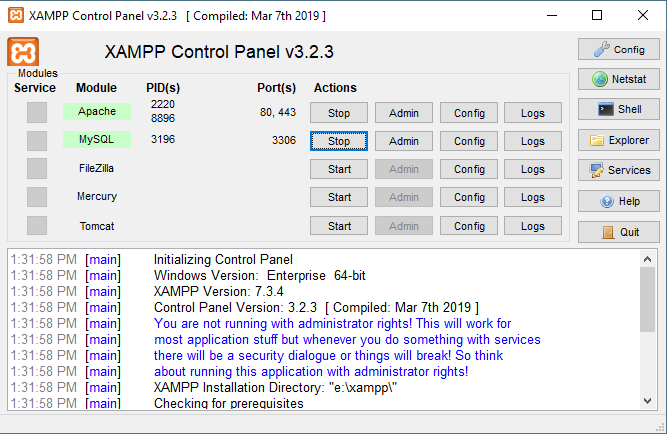
\includegraphics[scale=0.5]{figures/controlpanel}
\caption{XAMPP Control Panel}
\end{figure}

\item Jika sudah berjalan maka selanjutnya buka web browser kesayangan kita lalu ketikan https://localhost/phpmyadmin

 \begin{figure}[h]
\centering
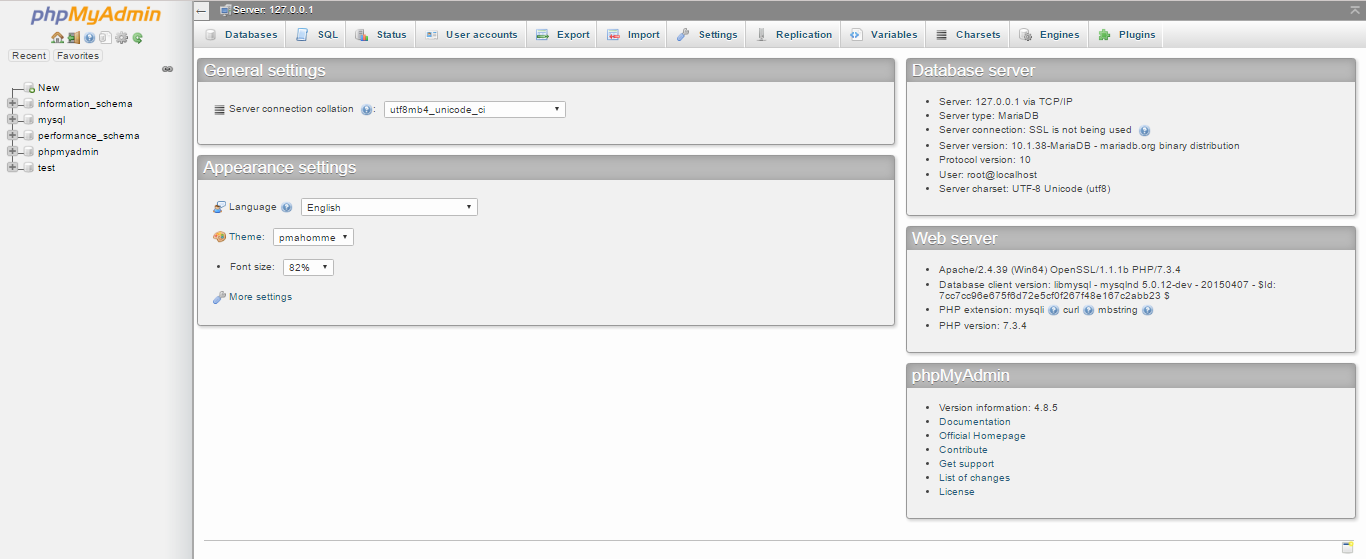
\includegraphics[scale=0.35]{figures/phpmyadmin}
\caption{Halaman Utama}
\end{figure}

\item Setelah itu, klik databases lalu ketikkan elban lalu klik create

 \begin{figure}[h]
\centering
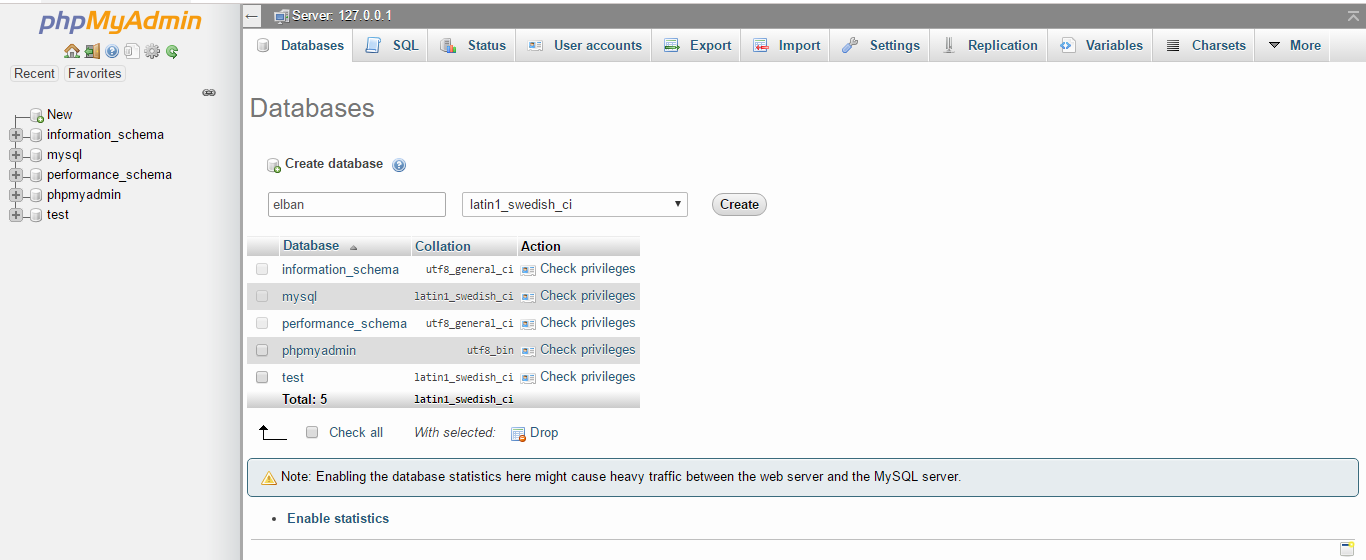
\includegraphics[scale=0.35]{figures/databases}
\caption{Create Database}
\end{figure}

\item Setelah database dibuat lalu belum ada table, klik SQL lalu masukan codingan berikut

\begin{lstlisting}
CREATE TABLE IF NOT EXISTS `logbook` (
  `id_logbook` int(10) NOT NULL,
  `tanggal` date NOT NULL,
  `petugas` varchar(100) NOT NULL,
  `vendor` varchar(100) NOT NULL,
  `penerbangan` varchar(100) NOT NULL,
  `kegiatan` varchar(500) NOT NULL,
  `point_kerusakan` varchar(200) NOT NULL,
  `target_pekerjaan` varchar(200) NOT NULL,
  `id_user` tinyint(1) NOT NULL
) ENGINE=InnoDB AUTO_INCREMENT=4 DEFAULT CHARSET=latin1;

--
-- Dumping data for table `logbook`
--

INSERT INTO `logbook` (`id_logbook`, `tanggal`, `petugas`, `vendor`, `penerbangan`, `kegiatan`, `point_kerusakan`, `target_pekerjaan`, `id_user`) VALUES
(2, '2019-03-31', 'M. Arif S, Vania & Rismayadi', 'Anto (CUPPS) Hisyam', 'Citylink KJT - KNO', 'PM di SCP 2 Inter Line 1', 'Master Clok Gate 4, XRAY BHS Internasional', 'Master Clock Gate 4', 12),
(3, '2019-03-28', 'M. Arif S & Vania', 'Anto (CUPPS) Hisyam', 'KJT - KNO (Cancelled)', 'PM', 'Master clock gate 4 off', 'Master CloCk gate 4', 12);

-- --------------------------------------------------------

--
-- Table structure for table `pegawai`
--

CREATE TABLE IF NOT EXISTS `pegawai` (
  `id_pegawai` int(10) NOT NULL,
  `pegawai` varchar(100) NOT NULL
) ENGINE=InnoDB AUTO_INCREMENT=16 DEFAULT CHARSET=latin1;

--
-- Dumping data for table `pegawai`
--

INSERT INTO `pegawai` (`id_pegawai`, `pegawai`) VALUES
(1, 'M. Arif S'),
(2, 'M. Arif S & Vania'),
(3, 'M. Arif S, Vania & Hafiz'),
(4, 'M. Arif S, Vania & Rismayadi'),
(5, 'M. Arif S & Hafiz'),
(6, 'M. Arif S & Rismayadi'),
(7, 'M. Arif S, Vania, Hafiz & Rismayadi'),
(8, 'Vania'),
(9, 'Vania & Hafiz'),
(10, 'Vania & Rismayadi'),
(11, 'Vania, Hafiz & Rismayadi'),
(12, 'Hafiz'),
(13, 'Hafiz & Rismayadi'),
(14, 'Rismayadi'),
(15, 'M. Arif S, Hafiz & Rismayadi');

-- --------------------------------------------------------

--
-- Table structure for table `user`
--

CREATE TABLE IF NOT EXISTS `user` (
  `id_user` tinyint(2) NOT NULL,
  `username` varchar(30) NOT NULL,
  `password` varchar(35) NOT NULL,
  `nama` varchar(50) NOT NULL,
  `alamat` varchar(150) NOT NULL,
  `hp` varchar(20) NOT NULL,
  `level` tinyint(1) NOT NULL
) ENGINE=InnoDB AUTO_INCREMENT=14 DEFAULT CHARSET=latin1;

--
-- Dumping data for table `user`
--

INSERT INTO `user` (`id_user`, `username`, `password`, `nama`, `alamat`, `hp`, `level`) VALUES
(1, 'admin', '21232f297a57a5a743894a0e4a801fc3', 'Luqman Nurfajri', 'Ciwarugotham', '089634530333', 1),
(13, 'vania', '081c2ce8528c443cc4be69d4096c9778', 'Vania R', 'Kertajati', '-', 1);

--
-- Indexes for dumped tables
--

--
-- Indexes for table `logbook`
--
ALTER TABLE `logbook`
  ADD PRIMARY KEY (`id_logbook`);

--
-- Indexes for table `pegawai`
--
ALTER TABLE `pegawai`
  ADD PRIMARY KEY (`id_pegawai`);

--
-- Indexes for table `user`
--
ALTER TABLE `user`
  ADD PRIMARY KEY (`id_user`);

--
-- AUTO_INCREMENT for dumped tables
--

--
-- AUTO_INCREMENT for table `logbook`
--
ALTER TABLE `logbook`
  MODIFY `id_logbook` int(10) NOT NULL AUTO_INCREMENT,AUTO_INCREMENT=4;
--
-- AUTO_INCREMENT for table `pegawai`
--
ALTER TABLE `pegawai`
  MODIFY `id_pegawai` int(10) NOT NULL AUTO_INCREMENT,AUTO_INCREMENT=16;
--
-- AUTO_INCREMENT for table `user`
--
ALTER TABLE `user`
  MODIFY `id_user` tinyint(2) NOT NULL AUTO_INCREMENT,AUTO_INCREMENT=14;
\end{lstlisting}

\end{enumerate}